\documentclass{article}
\usepackage[utf8]{inputenc}
\usepackage{graphicx}
\graphicspath{ {images/} }

\title{How I organize research code}
\author{Robby Parker}
\date{September 2022}

\begin{document}

\maketitle

\section{Motivation}
Computational research involves writing many different pieces of code.
Often, when writing a new piece of code, I find myself wondering where
to put it. And then wondering when it is ``good enough'' to be promoted.
This document presents and describes the different repositories that I
use to manage code for different projects, at different levels of
maturity.

\section{Different repositories}

\hspace{-2cm}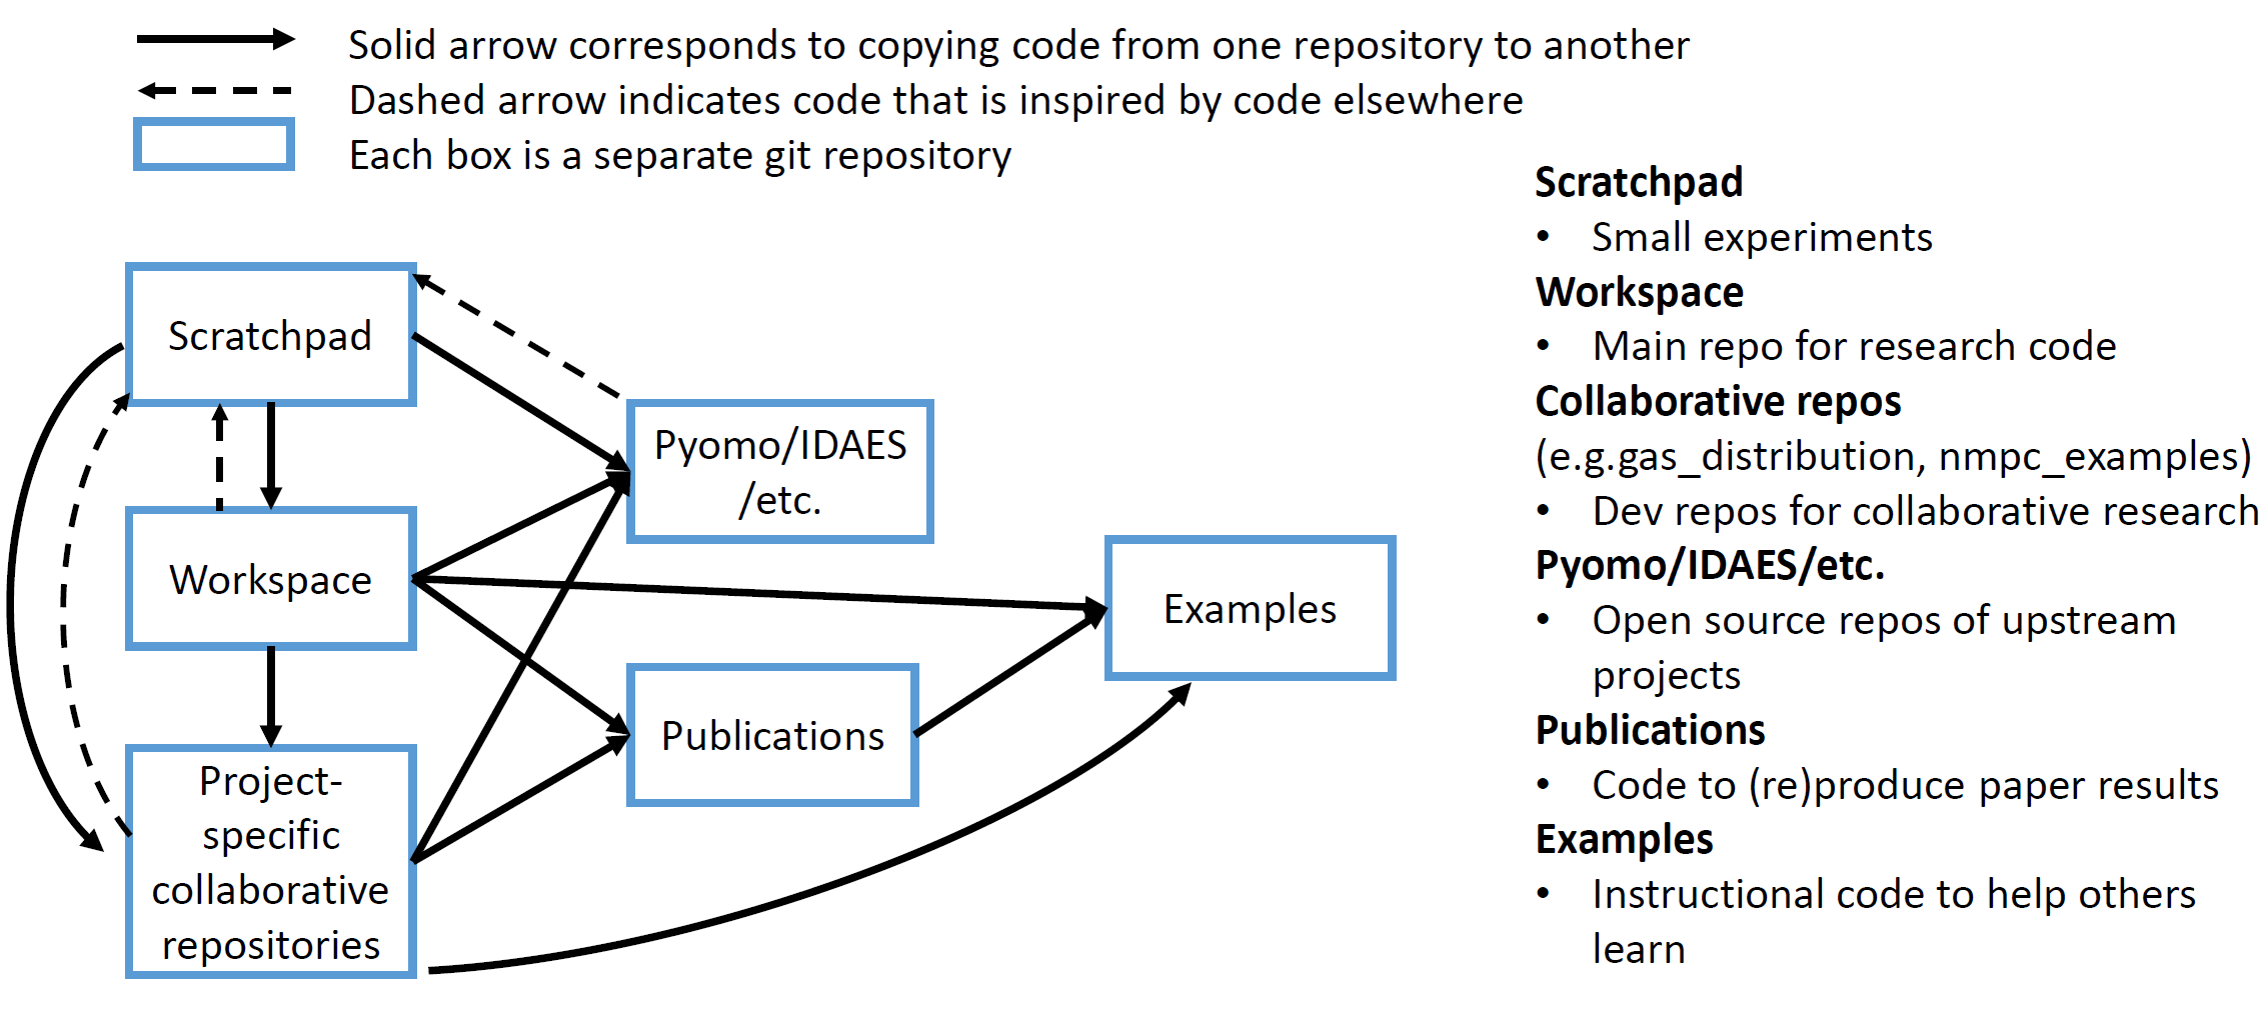
\includegraphics[width=16cm]{repo_diagram}

Most code starts out in workspace, either as a utility method/class,
implementation an algorithm, or model/case study.
It then gets promoted through one of several pathways:
\begin{itemize}
  \item Copied to the repo of an upstream open-source project (e.g. Pyomo,
    IDAES) for PR, review, and eventual merge
  \item Copied into its own repository for collaborative development
  \item Copied into a dedicated repository for publications when it is
    being used for paper results
  \item Copied into a dedicated repository for examples (of some tool
    or algorithm)
\end{itemize}

\section{Scratchpad}
\begin{itemize}
  \item Private repo
  \item Doesn't use branches
  \item Testing requirement: None
  \item Documentation requirement: None
\end{itemize}
A repository for running small examples, testing new features, and
debugging. I often use this to write a small script to test a new
Pyomo feature or test something while reviewing a PR.

\section{Workspace}
My main repository for research development.


\end{document}
